\subsection{Bridge}
\subsubsection{Định nghĩa}
Bridge pattern là một mẫu thiết kế thuộc nhóm cấu trúc (structural pattern) trong lập trình hướng đối tượng. Nó giúp tách biệt abstraction (abstraction) và implementation (implementation), cho phép chúng được phát triển độc lập và có thể thay đổi mà không ảnh hưởng đến nhau.
\subsubsection{Cách sử dụng}
Sử dụng Bridge Patern khi chúng ta muốn:
\begin{itemize}
    \item Khi bạn muốn tách rời abstraction và implementation để chúng có thể thay đổi một cách độc lập.
    \item Khi bạn muốn có khả năng mở rộng và thêm các implementation mới mà không ảnh hưởng đến abstraction hiện có.
\end{itemize}
\subsubsection{Cấu trúc}
Các thành phần chính:
\begin{itemize}
    \item Một interface hay abstract class định nghĩa các đối tượng liên quan.
    \item Một loạt các subclass kế thừa từ interface để tạo ra các loại sản phẩm.
    \item Một interface định nghĩa một cách hoạt động chung.
    \item Một loạt các class kế thừa từ interface để cụ thể hóa việc thực thi.
\end{itemize}
\begin{center}
    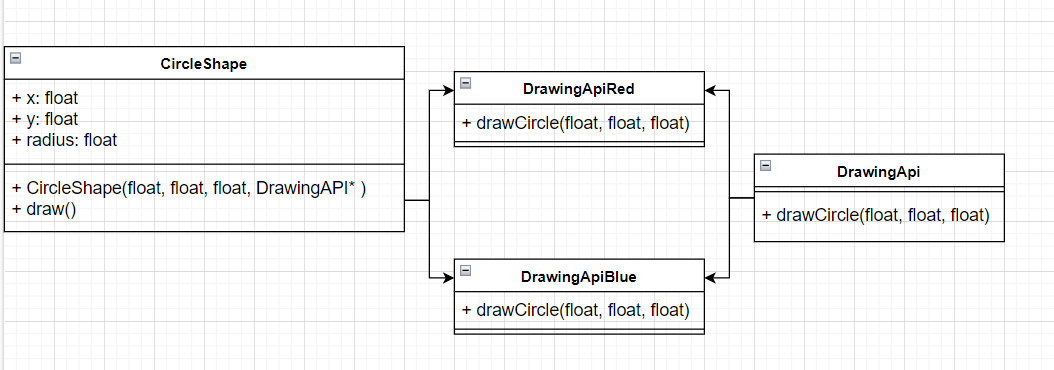
\includegraphics[scale=0.7]{image/structural/bridge.png}
\end{center}
\begin{itemize}
    \item Ở đây, CirceShape là một Concrete Class của Shape thuộc Abtraction Class, có thêm nhiều class như thế này vào không thành vấn đề.
    \item DrawingApi là một Implementation Class các Subclass của class này sẽ cụ thể thực hiện hành động như thế nào với các subclass của abstraction class. Bạn có thể thêm thoải mái các class như thế này.
\end{itemize}
\subsubsection{Ưu điểm và Nhược điểm}
Ta có các ưu và nhược điểm dễ thấy sau:\\\\
Ưu điểm:
\begin{itemize}
    \item Tách biệt abstraction và implementation, giúp giảm sự phức tạp và khả năng linh hoạt hơn trong việc thay đổi và mở rộng các thành phần.
    \item Các lớp abstraction và implementation có thể được mở rộng một cách độc lập, cho phép thêm mới các subclass mà không ảnh hưởng đến nhau.
\end{itemize}
Nhược điểm:
\begin{itemize}
    \item Đôi khi việc tách rời abstraction và implementation có thể tạo ra sự phức tạp thêm cho hệ thống nếu không được sử dụng một cách hợp lý.
\end{itemize}
\subsubsection{Code Example}
\begin{itemize}
    \item Có một loại hình duy nhấ là hình tròn.
    \item Có 2 cách vẽ với 2 màu khác nhau.
\end{itemize}
\begin{lstlisting}
#include <iostream>

// Abstraction
class Shape {
protected:
    class DrawingAPI* drawingAPI;

public:
    Shape(DrawingAPI* api) : drawingAPI(api) {}
    virtual void draw() = 0;
};

// Implementation
class DrawingAPI {
public:
    virtual void drawCircle(float x, float y, float radius) = 0;
};

// Concrete Implementation 1
class DrawingAPIRed : public DrawingAPI {
public:
    void drawCircle(float x, float y, float radius) {
        std::cout << "Red circle at (" << x << "," << y << ") radius " << radius << std::endl;
    }
};

// Concrete Implementation 2
class DrawingAPIBlue : public DrawingAPI {
public:
    void drawCircle(float x, float y, float radius) {
        std::cout << "Blue circle at (" << x << "," << y << ") radius " << radius << std::endl;
    }
};

// Refined Abstraction
class CircleShape : public Shape {
private:
    float x, y, radius;

public:
    CircleShape(float x, float y, float radius, DrawingAPI* api) : Shape(api), x(x), y(y), radius(radius) {}

    void draw() {
        drawingAPI->drawCircle(x, y, radius);
    }
};

int main() {
    DrawingAPIRed drawingAPIred;
    DrawingAPIBlue drawingAPIblue;

    CircleShape circle1(1, 2, 3, &drawingAPIred);
    CircleShape circle2(4, 5, 6, &drawingAPIblue);

    circle1.draw();
    circle2.draw();

    return 0;
}

\end{lstlisting}
Ở hàm main, ta thực hiện gọi 2 api để vẽ hình tròn với 2 màu khác nhau.\\
\newline
\textbf{Kết quả:}
\begin{lstlisting}
Red circle at (1,2) radius 3
Blue circle at (4,5) radius 6
\end{lstlisting}
\subsubsection{Các Pattern liên quan}
\begin{itemize}
    \item Adapter và Bride giống nhau về cấu trúc nhưng khác nhau về mục đích sử dụng.
    \item Abstract Factory: việc ghép nối này là hữu ích vì các Abstraction trong Bridge trong một số trường hợp chỉ có thể hoạt động được với các triển khai cụ thể nên việc đóng gói của Abstract Factory là cần thiết.
    \item Builder: Director giữ vai trò của Abstraction và các Builder giũ vai trò của Implementation.
\end{itemize}